\documentclass[SKL-MASTER.tex]{subfiles}
\begin{document}
\Large
	\subsection*{Finding the closest objects in the feature space}
	Sometimes, the easiest thing to do is to just find the distance between two objects. We just need
	to find some distance metric, compute the pairwise distances, and compare the outcomes to
	what's expected.
	\subsubsection*{Getting ready}
	\begin{itemize}
	\item A lower-level utility in scikit-learn is \texttt{sklearn.metrics.pairwise}. This contains server
	functions to compute the distances between the vectors in a matrix X or the distances
	between the vectors in X and Y easily.
	
	\item This can be useful for information retrieval. For example, given a set of customers with
	attributes of X, we might want to take a reference customer and find the closest customers to
	this customer. 
	\item In this scenario, we might want to rank customers by the notion of similarity measured
	by a distance function. The quality of the similarity depends upon the feature space selection
	as well as any transformation we might do on the space.\\ 
	\end{itemize}

	
\noindent	We'll walk through several different scenarios of measuring distance.
	\subsubsection*{Implementation}
	We will use the \texttt{pairwise\_distances} function to determine the "closeness" of objects.
	Remember that the closeness is really just similarity that we use our distance function
	to assess.
	
	First, let's import the pairwise distance function from the \textbf{metrics} module and create a
	dataset to play with:
	
	\begin{framed}
		\begin{verbatim}
		>>> from sklearn.metrics import pairwise
		>>> from sklearn.datasets import make_blobs
		>>> points, labels = make_blobs()
		\end{verbatim}
	\end{framed}
	This simplest way to check the distances is \texttt{pairwise\_distances}:
	\begin{framed}
		\begin{verbatim}
		>>> distances = pairwise.pairwise_distances(points)
		\end{verbatim}
	\end{framed}
	
	\noindent \texttt{distances} is an N x N matrix with 0s along the diagonals. In the simplest case, let's see the
	distances between each point and the first point:
	
	\begin{framed}
		\begin{verbatim}
		
		>>> np.diag(distances) [:5]
		
		array([ 0., 0., 0., 0., 0.])
		\end{verbatim}
	\end{framed}
	\begin{figure}[h!]
\centering
\includegraphics[width=0.7\linewidth]{images/distancematrix}
\end{figure}

	%========================================================%
	% % Chapter 3
	% % 103
	Now we can look for points that are closest to the first point in points:
	{\large
	\begin{framed}
		\begin{verbatim}
		>>> distances[0][:5]
		
		array([ 0., 11.82643041,1.23751545, 1.17612135, 14.61927874])
		\end{verbatim}
	\end{framed}
}
	Ranking the points by closeness is very easy with \texttt{np.argsort}:
	\begin{framed}
		\begin{verbatim}
		>>> ranks = np.argsort(distances[0])
		>>> ranks[:5]
		
		array([ 0, 27, 98, 23, 67])
		\end{verbatim}
	\end{framed}
	A useful characteristic of \texttt{argsort} is that now we can sort our points matrix to get the
	actual points:
	\begin{framed}
		\begin{verbatim}
		>>> points[ranks][:5]
	    array([[ 8.96147382, -1.90405304],
	           [ 8.75417014, -1.76289919],
		           [ 8.78902665, -2.27859923],
		           [ 8.59694131, -2.10057667],
		           [ 8.70949958, -2.30040991]])
		\end{verbatim}
	\end{framed}
	It's useful to see what the closest points look like. 
	%Other than some assurances, this works
	%as intended:
	
	\begin{figure}
		\centering
		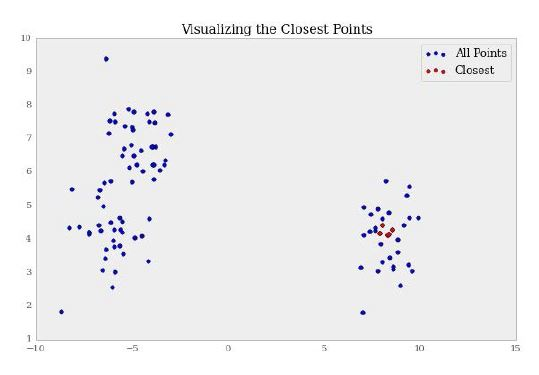
\includegraphics[width=0.8\linewidth]{SKL39-ClosestPoints}
		\caption{}
		\label{fig:SKL39-ClosestPoints}
	\end{figure}
	
	%========================================================%
	% % Building Models with Distance Metrics
	% % 104
	\newpage
	\subsubsection*{Theory : Euclidean Distance} % % How it works...
	Given some distance function, each point is measured in a pairwise function. The default is
	the Euclidian distance, which is as follows:
	
	if $p = (p1, p2,..., pn)$ and $q = (q1, q2,..., qn)$ are two points in Euclidean $n-$space, then the distance (d) from p to q, or from q to p is given by the Pythagorean formula:
	\[\mathrm{d}(\mathbf{p},\mathbf{q}) = \mathrm{d}(\mathbf{q},\mathbf{p}) \]\[ = \sqrt{(q_1-p_1)^2 + (q_2-p_2)^2 + \cdots + (q_n-p_n)^2} \]
	\[ = \sqrt{\sum_{i=1}^n (q_i-p_i)^2}.\]
	
	Verbally, this takes the difference between each component of the two vectors, squares the
	difference, sums them, and then takes the square root. This looks very familiar as we used
	something very similar to this when looking at the mean-squared error. If we take the square
	root, we have the same thing. In fact, a metric used often is root-mean-square deviation
	(RMSE), which is just the applied distance function.
	
	In Python, this looks like the following:
	\begin{framed}
		\begin{verbatim}
		
		>>> def euclid_distances(x, y):
		
		return np.power(np.power(x - y, 2).sum(), .5)
		>>> euclid_distances(points[0], points[1])
		
		11.826430406213145
		\end{verbatim}
	\end{framed}
	\subsubsection*{Other Distance Measures}
	There are several other functions available in scikit-learn, but scikit-learn will also use
	distance functions of SciPy. 
	% % At the time of writing this book, the scikit-learn distance functions support sparse matrixes. Check out the SciPy documentation for more information on the distance functions:
	\begin{enumerate}
		\item \texttt{cityblock}
		\item \texttt{cosine}
		\item \texttt{euclidean}
		\item \texttt{l1}
		\item \texttt{l2}
		\item \texttt{manhattan}
	\end{enumerate}
	\newpage
	\noindent \textbf{Worked Example} \\ We can now solve problems. For example, if we were standing on a grid at the origin, and the
	lines were the streets, how far will we have to travel to get to point (5, 5)?.
	\begin{framed}
		\begin{verbatim}
		>>> pairwise.pairwise_distances([[0, 2], [6, 6]], 
		  metric='cityblock')[0]
		
		array([ 0., 10.])
		\end{verbatim}
	\end{framed}
	%========================================================%
	%% - Chapter 3
	%% - 105
	%% - There's more...
	%%
	%%Using pairwise distances, we can find the similarity between bit vectors. It's a matter of finding
	%%the hamming distance, which is defined as follows:
	%%
	%%% % xi yi
	%%% % i
	%%% % I  
	%%
	%%Use the following command:
	%%\begin{framed}
	%%\begin{verbatim}
	%%>>> X = np.random.binomial(1, .5, size=(2, 4)).astype(np.bool)
	%%>>> X
	%%	array([[False, True, False, False],
	%%		   [False, False, False, True]], 
	%%		   dtype=bool)
	%%>>> pairwise.pairwise_distances(X, metric='hamming')
	%%array([[ 0. , 0.25],
	%%[ 0.25, 0. ]])
	%%\end{verbatim}
	%%\end{framed}
\end{document}\documentclass[SKL-MASTER.tex]{subfiles}
